\chapter{Tableaux}\label{tableaux}

\section{Composer un tableau}
\subsection{Créer des lignes et des colonnes}

Pour créer un tableau, aucun \jargon{package} supplémentaire n'est chargé.
L'environnement \texttt{tabular} sera utilisé en spécifiant un argument obligatoire composé d'une des trois lettres suivantes : \ordi l, \ordi c ou \ordi r. On peut inscrire plusieurs de ces lettres et une même lettre peut apparaître plusieurs fois.

Le nombre de lettres inscrites correspond simplement au nombre de colonne que contiendra le tableau. Dans chacune des colonnes, le texte pourra alors être aligné à gauche (\ordi l), centré (\ordi c) ou aligné à droite (\ordi r). Les lettres sont des \jargon{spécificateurs de colonnes}.

Ainsi, l'instruction \texttt{\textbackslash begin\{tabular\}\{rcl\}} permettra la création d'un tableau contenant trois colonnes, dont le texte sera aligné à droite dans la première colonne, centré dans la deuxième et enfin aligné à gauche dans la troisième. Il est inutile de spécifier le nombre de lignes.\bigskip


\begin{SideBySideExample}
    \begin{tabular}{rcl}
        Article & Couleur & Prix en euros \\[0.5cm]
        Pantalon & bleu & 25 \\
        Gants & blanc & 15 \\
            & Total & 40
    \end{tabular}
\end{SideBySideExample}
\bigskip

Comme pour l'environnement \texttt{align}, \verb!&! spécifie l'emplacement de l'alignement : autrement dit ce symbole sépare chaque colonne, y compris les colonnes vides.

La commande de changement de ligne \verb!\\! admet un argument optionnel qui sert à indiquer l'espace verticale que l'on veut insérer après cette ligne.

Afin de mieux visualiser les différentes lignes et colonnes, on peut ajouter des \jargon{filets} : la commande \verb!\hline! trace un \jargon{filet horizontal}.
Pour insérer un \jargon{filet vertical}, on peut inscrire une barre verticale \verb!|! entre les deux spécificateurs de colonnes concernés.\bigskip


\begin{SideBySideExample}
    \begin{tabular}{r||c|l}
        Article & Couleur & Prix en euros \\ \hline\hline
        Pantalon & bleu & 25 \\
        Gants & blanc & 15 \\ \hline
          & Total & 40
    \end{tabular}
\end{SideBySideExample}


\subsection{Fusionner des colonnes}

\LaTeX{} offre la commande \texttt{\textbackslash multicolumn}\texttt{<nombre-colonnes>}\texttt{<specificateur>}\texttt{<texte>} qui permet de fusionner horizontalement des colonnes.\bigskip

%{\NewFont
\begin{SideBySideExample}
    \begin{tabular}{r|c|l}
        \multicolumn{1}{c|}{Article} &
        Couleur & Prix en euros \\ \hline
        Pantalon & bleu & 25 \\
        Gants & blanc & 15 \\ \hline
        \multicolumn{2}{r}{Total :} & 40
    \end{tabular}
\end{SideBySideExample}
%}
\bigskip

\begin{info}
    On constate dans l'exemple précédent que la commande \texttt{\textbackslash multicolumn} permet non seulement de fusionner plusieurs colonnes mais aussi de modifier ponctuellement le spécificateur de colonne sur une cellule en particulier.
\end{info}

\subsection{Spécificateurs de colonne supplémentaires}

Les trois spécificateurs de base ne permettent pas de changement de ligne au sein d'une même cellule. De plus, on ne peut pas spécifier la largeur de la cellule. Le spécificateur \ordi{p}\{\texttt{<dim>}\} permet de composer une colonne en imposant une largeur : le texte est alors composé comme un paragraphe normal. \bigskip

%{\NewFont
\begin{SideBySideExample}
    \begin{tabular}{r|p{4.5cm}}
        Rectangle & Quadrilat\`ere dont les diagonales
        sont de m\^eme longueur et
        se coupent en leur milieu.\par
        Le rectangle est un parall\'elogramme.
    \end{tabular}
\end{SideBySideExample}
%}
\bigskip

Dans l'exemple précédent, on constate que les deux paragraphes sont alignés sur le haut de la cellule. On pourrait avoir envie de centrer verticalement ces paragraphes. On utilisera simplement \ordi{m}\{\texttt{<dim>}\} :\bigskip


\begin{SideBySideExample}
    \begin{tabular}{r|m{4.5cm}}
        Rectangle & Quadrilat\`ere dont les diagonales
        sont de m\^eme longueur et
        se coupent en leur milieu.\par
        Le rectangle est un parall\'elogramme.
    \end{tabular}
\end{SideBySideExample}

\bigskip

\begin{info}
    Dans l'exemple précédent, si l'on remplace \ordi{m\{4.5cm\}} par \ordi{b\{4.5cm\}}
    le texte sera aligné en bas verticalement.
\end{info}


\section{Les tableaux en mathématiques}\label{tabmath}
\subsection{L'environnement \texttt{array}}

Comme nous allons rapidement le voir, il peut être utile de composer des tableaux en mode mathématique (notamment en mode \jargon{hors texte}). Dans ce cas, on utilise dans le mode l'environnement \texttt{array} qui fonctionne comme \texttt{tabular} pour les commandes expliquées dans la section précédente.\bigskip

%{\NewFont
\begin{SideBySideExample}
    \[\begin{array}{rcl}
        f \colon \R & \rightarrow & \R_+ \\
                    x & \mapsto & x^2
    \end{array}\]
\end{SideBySideExample}
%}
\bigskip

\subsection{Les systèmes}\label{syst}

On avait constaté l'utilité des symboles étirables horizontalement. Servons-nous de \verb!\left\{! pour créer une grande accolade pour les systèmes :\bigskip

%{\NewFont
\begin{SideBySideExample}
    \[\left\{
    	\begin{array}{ccccccl}
    		2x & - & y & - & 3z & = & 1 \\
    		3x & + & 2y &  &  & = & -4 \\
    		-x &  &  & + & 6z & = & 22
    	\end{array}
    \right.\]
\end{SideBySideExample}
%}
\bigskip

\begin{info}
    \texttt{\textbackslash left} et \texttt{\textbackslash right} fonctionne toujours ensemble. Ici, on ne veut qu'une accolade à gauche. On utilise donc \texttt{\textbackslash left\textbackslash\{} mais la commande \texttt{\textbackslash right.} est nécessaire pour que la compilation ait lieu sans erreur.
\end{info}

%{\NewFont
\begin{SideBySideExample}
    \[\lvert x \rvert =
    \left\{
    	\begin{array}{cl}
    		-x & \text{si } x < 0 \\
    		x & \text{sinon}
    	\end{array}
    \right.\]
\end{SideBySideExample}
%}
\bigskip

Il existe un environnement permettant d'écrire des systèmes de façon rapide. Il s'agit de l'environnement \jargon{cases}. Il nécessite le \jargon{package} \texttt{amsmath} et aligne les équations à gauche.

\medskip

\begin{SideBySideExample}
    \[\begin{cases}
    2x+4y-5z+1=0\\
    x-y-5=0
    \end{cases}\]
\end{SideBySideExample}


\subsection{Les matrices}

Cette fois-ci, on peut penser à utiliser \verb!\left(! et \verb!\right)!\dots\bigskip

%{\NewFont
\begin{SideBySideExample}
    \[M = \left(
    	\begin{array}{ccc}
    		2 & -1 & 0 \\
            3 & 4 & 1 \\
            0 & 2 & 3
    	\end{array}
    \right)\]
\end{SideBySideExample}
%}
\bigskip

\dots mais en réalité des environnements spécifiques existent pour l'écriture des matrices. Entre autre, on retiendra les environnements \texttt{pmatrix} et \texttt{vmatrix} ainsi que la commande \texttt{\textbackslash bordermatrix}.\bigskip

%{\NewFont
\begin{SideBySideExample}
    \[M =
    	\begin{pmatrix}
    		2 & -1 & 0 \\
            3 & 4 & 1 \\
            0 & 2 & 3
    	\end{pmatrix}
    \]\medskip
    \[\det(M) =
    	\begin{vmatrix}
    		2 & -1 & 0 \\
            3 & 4 & 1 \\
            0 & 2 & 3
    	\end{vmatrix} = 29
    \]\medskip
    \[
        \bordermatrix{
            & f(e_1) & f(e_2) \cr
        e_1 & 1 & 2 \cr
        e_2 & 0 & 3 \cr}
    \]
\end{SideBySideExample}
%}
\bigskip

\section{Tableaux de signes et tableaux de variations}

Ici du allons utiliser l'environnement \texttt{tikzpicture} du \jargon{package} \texttt{TikZ}. Nous ne dirons rien sur ce \jargon{package} pour le moment mais nous reviendrons dessus lorsque nous traiterons les graphiques. Cependant, pour créer des tableaux de signes et des tableaux de valeurs, Alain \textsc{Matthes} a créé le \jargon{package} \texttt{tkz-tab} qui répond parfaitement bien à notre problème. Il faut donc penser dès à présent à ajouter \verb!\usepackage{tkz-tab}! au préambule.

\begin{info}
    Selon l'installation effectuée, il est possible que \texttt{tkz-tab} ne soit pas présent dans votre distribution. Vous vous en rendrez rapidement compte en compilant le premier exemple. La documentation de ce \jargon{package} est également une source à consulter absolument.
\end{info}

\subsection{Tableaux de signes}

%{\NewFont
\begin{CenterExample}
    \textbf{Tableau de signes :}\par
    \begin{tikzpicture}
        \tkzTabInit[nocadre,espcl=1.5,lgt=2.5]%
            {$x$/0.75,Signe de \\ $x+2$/1.5,Signe de \\ $x^2-1$/1.5,%
            signe du \\ produit/1.5,signe du \\ quotient/1.5}%
            {$-\infty$,$-2$,$-1$,$1$,$+\infty$}
        \tkzTabLine{,-,z,+,t,+,t,+}
        \tkzTabLine{,+,t,+,z,-,z,+}
        \tkzTabLine{,-,z,+,z,-,z,+}
        \tkzTabLine{,-,z,+,d,-,d,+}
    \end{tikzpicture}
\end{CenterExample}
%}
\bigskip

Un tableau de signes ou de variations commencera toujours par \texttt{\textbackslash tkzTabInit} dont voilà la syntaxe :
\begin{center}
    \texttt{\textbackslash tkzTabInit}[\texttt{<options>}]\{\texttt{<première colonne>}\}\{\texttt{<première ligne>}\}
\end{center}

 En option est spécifié que le cadre autour du tableau ne doit pas être dessiné, que l'espace entre les valeurs de la première ligne est réglée par le paramètre \verb!espcl! et que la largeur de la première colonne est réglée par le paramètre \verb!lgt!.
 
 Par défaut les valeurs de \verb!espcl! et \verb!lgt! sont réglées à \np[cm]{2}.
 
 Il existe également d'autres options :
 
$\star$ \verb!deltacl! : marge avant le premier antécédent et après le dernier, réglée à \np[cm]{0,5} par défaut,

$\star$ \verb!lw! : épaisseur des lignes du tableau, réglée à \np[pt]{0,4} par défaut,

$\star$ \verb!nocadre! : pour enlever le cadre entourant le tableau ; par défaut, on encadre le tableau

$\star$ \verb!color! : booléen qui autorise la couleur

$\star$ \verb!colorC! : couleur de la première colonne, réglée à \texttt{white} par défaut

$\star$ \verb!colorL! : couleur de la première ligne, réglée à \texttt{white} par défaut

$\star$ \verb!colorT! : couleur de la partie centrale, réglée à \texttt{white} par défaut

$\star$ \verb!colorV! : couleur de la case de la variable, réglée à \texttt{white} par défaut

 Ensuite, on énumère les différentes lignes de la première colonne : \texttt{nom de la ligne}\verb!/!\texttt{hauteur de la ligne}. Le \texttt{nom de la ligne} accepte des changements de lignes à l'aide de \verb!\\! et on passe d'une ligne à l'autre en utilisant la virgule.

 Enfin, dans le dernier argument, on écrit les valeurs de la première ligne en les séparant par une virgule.\medskip

 Pour finir, pour chaque ligne, on écrit les signes par la commande \texttt{\textbackslash tkzTabLine}. La lettre \verb!t! crée un filet vertical en pointillés et la lettre \verb!z! fait la même chose en ajoutant un zéro. La lettre \verb!d! insère une double-barre pour les valeurs interdites.

 \begin{info}
    Si on a besoin d'écrire des nombres décimaux, on prendra soin de les écrire entre accolades pour que la virgule ne crée pas de conflit : \ordi{\$\{1,5\}\$}.
 \end{info}

 \subsection{Tableaux de variations}

 %{\NewFont
\begin{CenterExample}
    \textbf{Tableau de variations :}\par
     \begin{tikzpicture}
        \tkzTabInit[nocadre,espcl=2,lgt=2.5]
        {$x$/0.75,Variations \\ de $f$/1.75}
        {$-3$,$-1$,$1$,$4$}
        \tkzTabVar{+/$6$,-D+/$-\infty$/$+\infty$,-/,+/$-5$}
    \end{tikzpicture}
\end{CenterExample}
%}
\bigskip

Il nous suffit ici de commenter la commande \texttt{\textbackslash tkzTabVar} : pour chaque valeurs de $x$ indiquée sur la première ligne, on peut préciser une valeur précédée du signe \verb!+/! pour dire que la valeur sera écrite \og en haut\fg{} ou bien \verb!-/! pour dire que la valeur sera écrite \og en bas \fg{}. Des flèches relieront alors automatiquement les différentes valeurs :
\begin{center}
    \texttt{\textbackslash tkzTabVar}{\tt\{}\texttt{<+ ou ->}{\tt/}\texttt{<valeur>} , \texttt{<+ ou ->}{\tt/}\texttt{<valeur>} , ...{\tt\}}
\end{center}

\begin{info}
    Pour la double-barre avec des valeurs indiquées avant et après celle-ci, on notera {\tt -D+/\texttt{<valeur>}/\texttt{<valeur>}} ou bien {\tt +D-/\texttt{<valeur>}/\texttt{<valeur>}}.
\end{info}

\subsection{Un mélange}
Et voilà maintenant ce que l'on peut obtenir :

\vspace*{-12pt}
% {\NewFont
\begin{CenterExample}
    \begin{tikzpicture}
        \tkzTabInit[nocadre,espcl=2,lgt=2.5]%
            {$x$/0.75,signe de \\ $f'(x)$/1.5,Variations \\ de $f$/1.75}%
            {$-3$,$-1$,$1$,$4$}
        \tkzTabLine{,+,z,-,z,+}
        \tkzTabVar{-/$-\infty$,+/,-/,+/$+\infty$}
    \end{tikzpicture}
\end{CenterExample}
%}

\subsection{Un dernier exemple}

Avec l'instruction \verb!\tkzTabIma! qui permet des images intermédiaires.

\color{blue}\rule{9cm}{1pt}\color{black}
\vspace*{-12pt}

\begin{small}
\begin{verbatim}
1. \begin{tikzpicture}
2. \tkzTabInit[color,lgt=2.5,espcl=3,colorC=blue!20,colorV=blue!20]%
3. {$t$/1,Variations\\ de $f$/2,Variations\\ de $g$/2}%
4. {$-1$,$0$,$1$,$2$}
5. \tkzTabVar{-/$-5$,+/$0$,-/$-1$,+/$4$}
6. \tkzTabVar{-/$-5$,R/,R/,+/$4$}
7. \tkzTabIma[draw]{1}{4}{2}{$0$}
8. \tkzTabIma[draw]{1}{4}{3}{$3$}
9. \end{tikzpicture}
\end{verbatim}
\end{small}
\vspace*{-12pt}

\color{blue}\rule{9cm}{1pt}\color{black}

\begin{center}
\begin{tikzpicture}
\tkzTabInit[color,lgt=2.5,espcl=3,colorC=blue!20,colorV=blue!20]%
{$t$/1,Variations\\ de $f$/2,Variations\\ de $g$/2}%
{$-1$,$0$,$1$,$2$}
\tkzTabVar{-/$-5$,+/$0$,-/$-1$,+/$4$}
\tkzTabVar{-/$-5$,R/,R/,+/$4$}
\tkzTabIma[draw]{1}{4}{2}{$0$}
\tkzTabIma[draw]{1}{4}{3}{$3$}
\end{tikzpicture}
\end{center}

\danger Pour placer une image entre deux autres, il faut que les deux images extrêmes existent\dots

Il ne faut donc pas utiliser une image qui a été remplacée par R\dots


\section{Complément : le tableur}

Le \jargon{package} \texttt{pas-tableur} de Stéphane \bsc{Pasquet} permet d'imiter l'apparence d'un tableur. Cependant, il n'effectue pas de calcul automatique comme dans un tableur (pour cela, on pourra jeter un {\oe}il sur le \jargon{package} \texttt{spreadtab}). Une fois encore, ce \jargon{package} utilise \texttt{TikZ} et son environnement \texttt{tikzpicture}.

La première commande à retenir est la suivante :
\begin{center}
    \texttt{\textbackslash tableur}[\texttt{<nombres-lignes>}]\{\texttt{<colonnes>}\}
\end{center}

L'argument \texttt{<colonnes>} permet de spécifier les lettres des colonnes utilisées soit une par une, soit en utilisant un \og intervalle \fg{}.

Ensuite, 
\begin{center}\texttt{\textbackslash celtxt}[\texttt{<options>}]\{\texttt{<colonne>}\}\{\texttt{<ligne>}\}\{\texttt{<texte>}\}\end{center} 
permet d'écrire un texte dans la cellule définie par \texttt{<colonne>} et \texttt{<ligne>}. Parmi les options, \verb!l!, \verb!c! et \verb!r! sont utilisées pour l'alignement du texte. Des formules commençant par le signe \verb!=! peuvent être écrites et le texte peut être mis en forme en utilisant les commandes correspondantes.

Et enfin, les commandes \texttt{\textbackslash selecCell} et \texttt{\textbackslash multiSelec} permettent de mettre en couleur des cellules sélectionnées. Les exemples suivants vous montrent comment :\bigskip

%{\NewFont
\begin{SideBySideExample}
    \begin{tikzpicture}
        \tabcolwidth{1cm}
        \tableur{A,D,T}
    \end{tikzpicture}\bigskip

    \begin{tikzpicture}
        \tabcolwidth{2cm}
        \tableur[3]{A,B,C}
        \multiSelec{A-2}{B-3}
    \end{tikzpicture}\bigskip

    \begin{tikzpicture}
        \tabcolwidth{1.5cm}
        \tableur[3]{A-D}
        \celtxt[c]{A}{1}{\itshape x}
        \celtxt[r]{A}{2}{0}
        \celtxt[r]{A}{3}{1}
        \celtxt[c]{B}{1}{\itshape f(x)}
        \celtxt{B}{2}{=A2*A2}
        \selecCell{B}{2}
    \end{tikzpicture}
\end{SideBySideExample}